% Figura cuerpo B1: el error adaptativo es sistemático; el racional cambia de signo y se compensa
\documentclass[tikz,border=3pt]{standalone}
\usepackage[T1]{fontenc}
\usepackage[utf8]{inputenc}
\usepackage{amsmath}
\usetikzlibrary{arrows.meta,calc,positioning}
\begin{document}
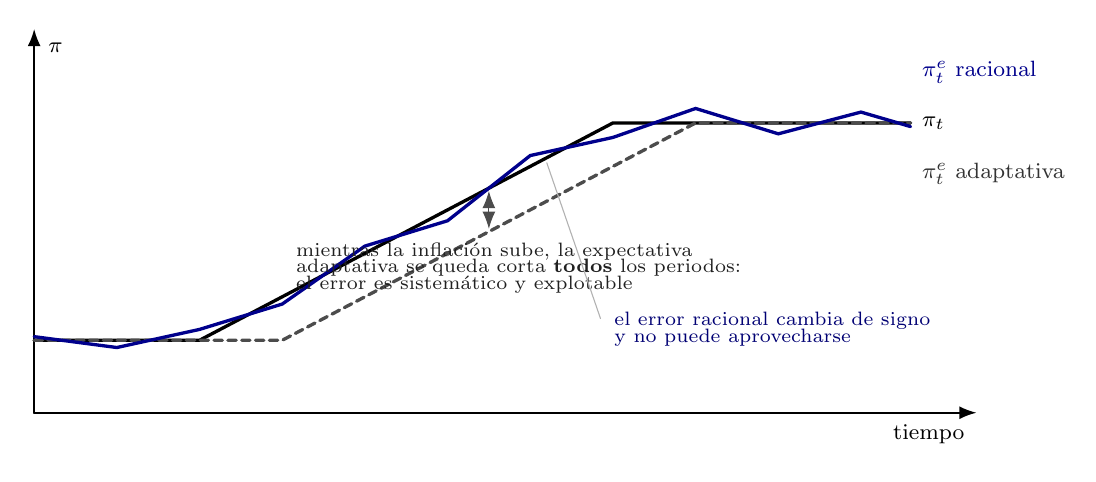
\begin{tikzpicture}[x=1.05cm, y=0.46cm, >={Latex[length=2.2mm]}, line cap=round, font=\footnotesize]
  \draw[->, thick] (0,0) -- (11.4,0) node[below left=1pt]{tiempo};
  \draw[->, thick] (0,0) -- (0,10.6) node[below right=2pt]{$\pi$};
  % Inflacion observada
  \draw[very thick] (0,2) -- (2,2) -- (7,8) -- (10.6,8);
  \node[anchor=west, inner sep=1pt] at (10.7,8) {$\pi_t$};
  % Expectativa adaptativa: la de ayer
  \draw[very thick, gray!60!black, densely dashed] (0,2) -- (3,2) -- (8,8) -- (10.6,8);
  \node[anchor=west, inner sep=1pt, gray!40!black] at (10.7,6.6) {$\pi^{e}_t$ adaptativa};
  % Expectativa racional: error que cambia de signo
  \draw[very thick, blue!55!black] plot coordinates
    {(0,2.1) (1,1.8) (2,2.3) (3,3.0) (4,4.6) (5,5.3) (6,7.1) (7,7.6) (8,8.4) (9,7.7) (10,8.3) (10.6,7.9)};
  \node[anchor=west, inner sep=1pt, blue!55!black] at (10.7,9.4) {$\pi^{e}_t$ racional};
  % Brecha sistematica
  \draw[<->, gray!60!black, shorten >=1pt, shorten <=1pt] (5.5,6.2) -- (5.5,5.0);
  \node[anchor=west, align=left, font=\scriptsize, gray!25!black] at (3.05,4.0)
    {mientras la inflación sube, la expectativa\\[-2pt]adaptativa se queda corta \textbf{todos} los periodos:\\[-2pt]el error es sistemático y explotable};
  \node[anchor=west, align=left, font=\scriptsize, blue!45!black] at (6.9,2.3)
    {el error racional cambia de signo\\[-2pt]y no puede aprovecharse};
  \draw[gray!60] (6.85,2.6) -- (6.2,6.9);
\end{tikzpicture}
\end{document}
